\section{Evaluation}
\label{sect:evaluation}

We have implemented a \sysname prototype as a Django web application
that features the REST API presented in Section~\ref{sect:fairtest}.
We evaluated our prototype by using it to uncover {\it privacy bugs}
in the pricing policy of the ``Staples Inc.'', as described by the
Wall Street Journal in 2012. We sought answer to the following three
questions:

\begin{enumerate}
  \item[{\bf Q1}] Can \sysname uncover {\em privacy bugs} for
    a pricing policy similar to the policy of the ``Staples Inc.''
    online store?
  \item[{\bf Q2}] What is the impact of {\em privacy bugs} in the outputs
    shown to users?
  \item[{\bf Q3}] What is impact of pricing policies on {\em privacy bugs}?
    Are {\em privacy bugs} inherent to any pricing policy, or are
    dependant on pricing policies?
\end{enumerate}

\subsection{\normalsize Methodology}
Our experimental evaluation of \sysname consists of the following three steps:

\begin{enumerate}
  \item
  Generate one million synthetic users that are spread accross the
  areas corresponding to 40,000 US zip-codes. These synthetic users
  have four attributes: zip-code, race, sex, and income, and match
  the demographic characteristics of the US population, according to
  the US Census Bureau~\cite{CensusBureau}, as of May 3, 2014.
  \footnote{
    The infrastructure necessary for generating syntetic users is
    provided by a project of the ``Advanced Distributed Systems'' course,
    tought by professor Roxana Geambasu, Spring 2015. The developers of the
    project are Z. Zhou, Z. Wan, and X. Ma.
  }

  \item
  Use the users generated in Step 1 to simulate one million user-visits on
  an online store with a pricing policy similar to the one that the
  ``Staples Inc.'' online store implements. After each visit,
  register to \sysname the respective synthetic user along with the ouput
  received.

  \item
  Query \sysname's web interface to uncover any strong correlation between
  outputs and protected user attributes, i.e., race, income, and sex.
\end{enumerate}

Since user-attributes match the demographics of the US popation,
race, sex, and income are assigned values that depend on the zip-code. Because
the later defines the area in which a user lives. In other words, user's race,
sex, and income correlate with user's zip-code, but not amongst each other.
Each synthetic user has
one of the following seven races: ``White'', ``Hispanic'', ``African
American'', ``Indian or Alaskan'', ``Asian'', ``Pacific Islander'', ``Other'',
and ``Two or More''. Also, each user is either ``Male'' or ``Female''. Finally,
each user has an income the lies into one of the following seven ranges:
``less then $\$5,000$'', ``more than $\$5,000$'', ``more than $\$10,000$'',
``more than $\$20,000$'', ``more than $\$40,000$'', ``more than $\$80,000$'',
``more than $\$160,000$'', ``more than $\$320,000$''.

\subsection{\normalsize Uncovering {\em Privacy Bugs}}
\label{sect:uncovering}
In this section we use \sysname to evaluate the {\em statistical parity}
of one million synthetic users that visit an online store which
implements a pricing policy summarized by the following rule:
{\it if a user's distance from a competitor's store
(``OfficeDepot \& OfficeMax'') is less than 20 miles, show a low price;
otherwise, show a high price.}
To evaluate {\em statistical parity} of users, we measure the dependency of
the delta of condition~\ref{eq:StatisticalParity} (introduced
in Section~\ref{sect:statparity}) on user's location. We group users
based on (a) income, (b) race, and (c) sex, and examine potential
violations of condition~\ref{eq:StatisticalParity} for $\epsilon=0.05$ and
output being ``high'' price.
Figure~\ref{fig:Deltas} shows the deltas
for user's race, income, and sex, as a function of price engine's dependency
on user' s location. When price engine's dependency on users location is zero,
all users receive random prices. When price engine's dependency on users
location is 100\%, all users receive prices strictly based on the rule
introduced in the previous paragraph.


Figure~\ref{fig:DeltasIncome} reveals that when users are grouped according to
their income, {\em statistical parity} is not dependant on user's location,
except for users with annual income more than \$320,000. Users whose income
lie in the later
categorie are treated differently (favorably or unfavorably) than the rest,
and their location correlates with the outputs (i.e., prices) they receive.
Figure~\ref{fig:DeltasRace} indicates that when users are groupped according
to their race, {\em statistical parity} is not dependant on user's location,
unless the user is an ``Indian American''. This signals that ``Indian
Americans'' are treated differently (favorably or unfavorably) than the rest.
Given the fact that both user's race and user's income are a protected
attribute, one can use \sysname's reports to conclude that the impelented
pricing policy imposes an undesirable privacy bug, which is
summarized as follows: ``If a user is an Indian American or has an income more
than \$320,000 he or she will consistently be treated diffently than others.''
On the other hand, Figure~\ref{fig:DeltasSex} indicates when users are grouped
according to their sex, {\em statistical parity} is independent of location,
and therefore males are treated similarly to females.

\begin{figure*}[t]
{
  \subfigure[Income]{
    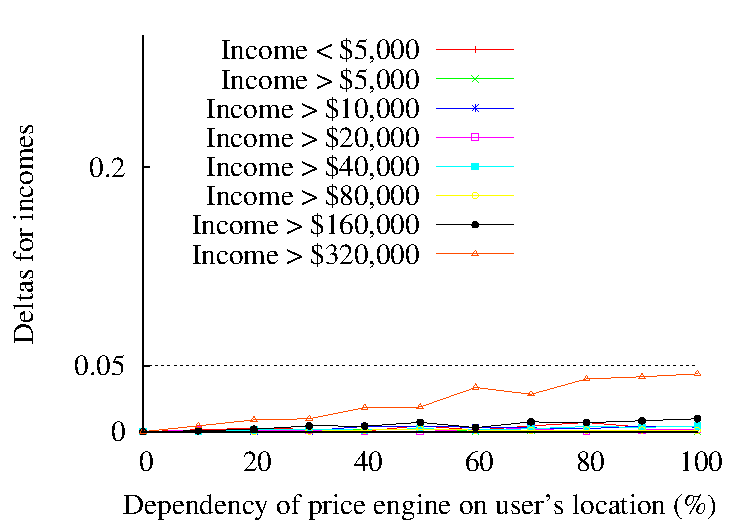
\includegraphics[width=0.33\textwidth]
    {\detokenize{results/income_discrimination_on_location_dependency}}
    \label{fig:DeltasIncome}
  }
  \subfigure[Race]{
    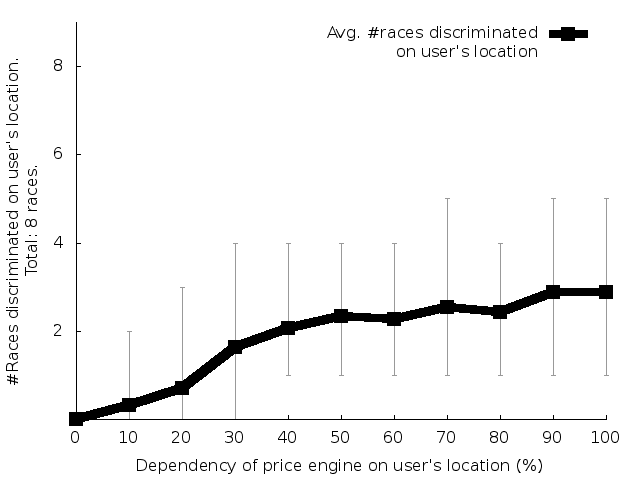
\includegraphics[width=0.33\textwidth]
    {\detokenize{results/race_discrimination_on_location_dependency}}
    \label{fig:DeltasRace}
  }
  \subfigure[Sex]{
    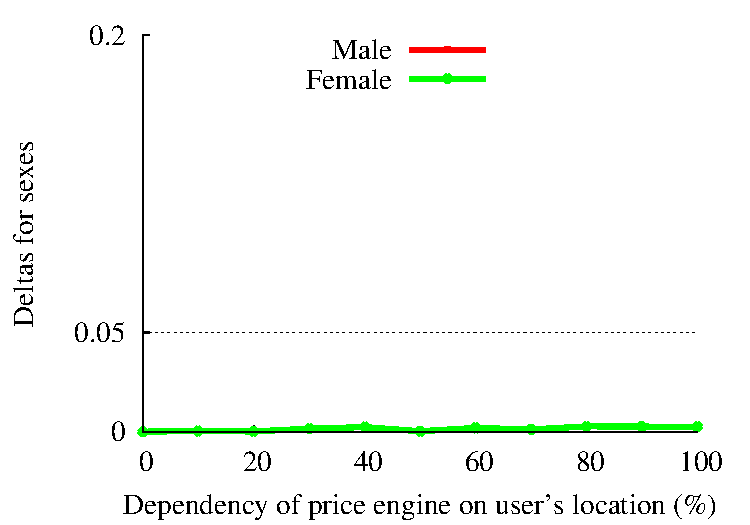
\includegraphics[width=0.33\textwidth]
    {\detokenize{results/sex_discrimination_on_location_dependency}}
    \label{fig:DeltasSex}
  }
  \caption{\textbf{Statistical parity and its dependency on user's location.}
          Shows the dependency of statistical parity on user's location,
          when users are grouped based on (a) income, (b) race, and (c) sex.
          Figures (a) and (b) reveal that when users are grouped according to
          income and race, statistical parity correlates for some groups with
          the dependency of the price engine on user's location. While Figure
          (c) reveals that statistical parity is independent of user's location
          when users are grouped based on sex.
  }
  \label{fig:Deltas}
}
\end{figure*}

\begin{figure*}[t]
{
  \subfigure[Income]{
    \includegraphics[width=0.33\textwidth]
    {\detokenize{results/income_discrimination_on_proportional}}
    \label{fig:IncomeDiscriminationProportional}
  }
  \subfigure[Race]{
    \includegraphics[width=0.33\textwidth]
    {\detokenize{results/race_discrimination_on_proportional}}
    \label{fig:RaceDiscriminationProportional}
  }
  \subfigure[Sex]{
    \includegraphics[width=0.33\textwidth]
    {\detokenize{results/sex_discrimination_on_proportional}}
    \label{fig:SexDiscriminationProportional}
  }
  \caption{\textbf{Prices shown to users and their dependency on income,
          race, and sex.} Shows the proportion of high versus low
          prices shown to users based on (a) income, (b) race, and (c) sex.
          Figure (a) reveals that a users with annual income less than
          \$5,000 receives proportionaly more high prices than a user with
          annual income more than \$320,000. Figure (a) indicates that an
          Indian American or an Alaskan users receives notably more high prices
          than any other user. This raises a consern, since as shown in
          Figure~\ref{fig:IncomePerRace}, an Indian American or an Alaskan
          user has on average a considerably lower annual income than a
          white American user. Figure (c) shows that male and female users
          receive approximately the same proportion of high versus
          low prices.
  }
  \label{fig:DiscriminationProportional}
}
\end{figure*}
\begin{figure}[t]
 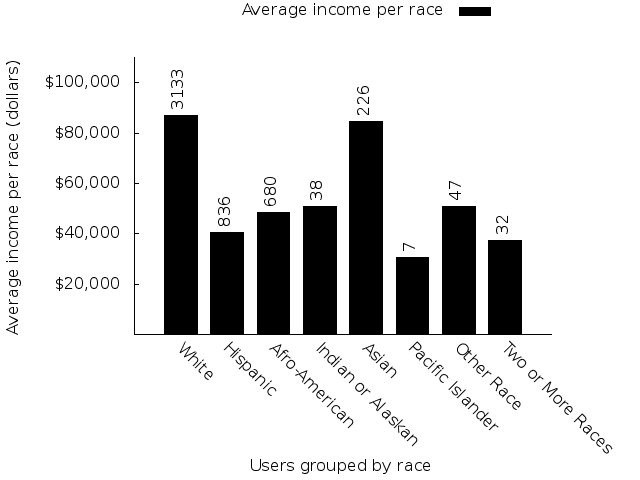
\includegraphics[width=0.49\textwidth]
  {\detokenize{results/income_per_race}}
  \caption{\textbf{Average annual income per race.} An Indian or an Alaskan user has
           a considerably lower income than a white American, and yet, as shown in
           Figure~\ref{fig:IncomeDiscriminationProportional}, he or she receives
           proportionally more high prices.
  }
  \label{fig:IncomePerRace}
\end{figure}






\subsection{\normalsize Measuring the Impact of {\em Privacy Bugs}}
Having concluded that the implemented pricing policy violates {\em statistical
parity} of users, i.e., introduces {\em privacy bugs}, we now investigate the
impact of these bugs. To this end, we examine whether users are treated
favorably or unfavorably by measuring the proportion of ``high'' vesus ``low''
prices shown to users. Figure~\ref{fig:DiscriminationProportional} shows in
percentage the proportion of ``high'' vesus ``low'' prices shown to users
grouped by (a) race, (b) income, and (c) sex. On top of each bar the raw number
of members of the respective group is shown.

Figure~\ref{fig:IncomeDiscriminationProportional} shows that for each income
group around 6\% of users receive ``high'' prices (the rest receive ``low''
prices), except the income group which consists of users with annual income
more than \$320,000. Recall that based on Figure~\ref{fig:DeltasIncome}, we
had already concluded that users with annual income more than \$320,000 are
treated differently that the rest. Additionally,
Figure~\ref{fig:IncomeDiscriminationProportional} shows that users with
annual income more than \$320,000 are treated favorably compare to the rest.
Note that a user with annual income less than \$5,000 is more probable to
receive a high price, than a user with annual income more than \$320,000.
Clearly this is a very poor -- yet unintentional -- algorithmic decision imposed
by a privacy bug which is difficult to foresee without the aid of \sysname.


Figure~\ref{fig:RaceDiscriminationProportional} indicates that the
percentage of ``high'' prices shown to ``Indian Americans and Alaskans'' is
notably higher than any other race. Recall that by analyzing
Figure~\ref{fig:DeltasRace}, we had already concluded that
``Indian Americans and Alaskans'' are treated diffently than the rest.
In addition, Figure~\ref{fig:RaceDiscriminationProportional} reveals that
``Indian Americans and Alaskans'' are treated unfavorably, since they are
more probable to receive a ``high'' price, than the rest. This is also a very
poor algorithmic decision, because as shown in Figure~\ref{fig:IncomePerRace},
``Indian Americans and Alaskans'' have a low annual income on average. In
other words, the enforced pricing policy consistently shows more
``high'' prices to populations with lower annual income.


\subsection{\normalsize Measuring the Impact of Pricing Policies}
Finally, we examine the impact of different pricing policies on the presence
of {\em privacy bugs}, and seek to understand how algorithmic decision
affect {\em privacy bugs}. To achieve this, we modify the pricing policy
to now abide by the following rule: {\it if a user's distance from a
competitor's store (``OfficeDepot \& OfficeMax'') is less than 10 miles,
show a low price; otherwise, show a high price.} Then, we compare the outputs
shown to users in this case, against the outputs shown to users with the policy
introduced in Section~\ref{sect:uncovering}. Note that the only modification 
is the change on the competitor's distance from 20 miles to 10 miles.

Figure~\ref{fig:DiscriminationProportionalAdditional} show that after
applying the new  pricing policy more users receive ``high'' prices
compared to Figure~\ref{fig:DiscriminationProportional}. This is expected
since we apply a stricter policy that shows ``low'' if the competitor's
stores are within 10 miles,  instead of 20 miles. Notably, however, Indian Americans
and Alaskans are still the most unfavorably treated populations. Also, users
with annual income more than \$320,000 are still the most favorably treated
poulation. This indicates that despite variations of the pricing policies,
there are inherent correlations between user attributes that are transparent
to developers, had it not been \sysname. Hence, we believe that \sysname
helps increase developers transparency of data use and provide some understanding
of the policies applyied on the data.



\begin{figure*}[t]
{
 \subfigure[Income]{
    \includegraphics[width=0.33\textwidth]
    {\detokenize{results/misc/income_discrimination_on_proportional}}
    \label{fig:IncomeDiscriminationProportionalAdditional}
  }
  \subfigure[Race]{
    \includegraphics[width=0.33\textwidth]
    {\detokenize{results/misc/race_discrimination_on_proportional}}
    \label{fig:RaceDiscriminationProportionalAdditional}
  }
  \subfigure[Sex]{
    \includegraphics[width=0.33\textwidth]
    {\detokenize{results/misc/sex_discrimination_on_proportional}}
    \label{fig:SexDiscriminationProportionalAdditional}
  }
  \caption{\textbf{NEWPrices shown to users and their dependency on income,
          race, and sex.} Shows the proportion of high versus low
          prices shown to users based on (a) income, (b) race, and (c) sex.
          Figure (a) reveals that a users with annual income less than
          \$5,000 receives proportionaly more high prices than a user with
          annual income more than \$320,000. Figure (a) indicates that an
          Indian American or an Alaskan users receives notably more high prices
          than any other user. This raises a consern, since as shown in
          Figure~\ref{fig:IncomePerRace}, an Indian American or an Alaskan
          user has on average a considerably lower annual income than a
          white American user. Figure (c) shows that male and female users
          receive approximately the same proportion of high versus
          low prices.
  }
  \label{fig:DiscriminationProportionalAdditional}
}
\end{figure*}



